\section{Aritmética en C}\label{aritmuxe9tica-en-c}

\begin{frame}{Operadores Aritméticos}

\begin{longtable}[c]{@{}cccc@{}}
\toprule\addlinespace
Operación C & Operador aritméco & Expresiólgebraica & Expresión C
\\\addlinespace
\midrule\endhead
Suma & + & f + 7 & f + 7
\\\addlinespace
Resta & - & p - c & p - c
\\\addlinespace
Multiplicación & * & bm o \texttt{b*m} & \texttt{b*m}
\\\addlinespace
División & / & x/y & x / y
\\\addlinespace
Módulo & \% & r mod s & r \% s
\\\addlinespace
\bottomrule
\end{longtable}

\end{frame}

\begin{frame}{Operadores Aritéticos}

\begin{figure}[htbp]
\centering
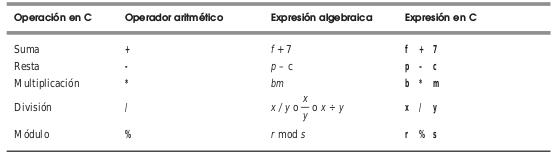
\includegraphics{operadores-aritmeticos.jpg}
\caption{Operadores Aritméticos}
\end{figure}

\end{frame}

\begin{frame}{Precedencia de Operadores}

\begin{figure}[htbp]
\centering
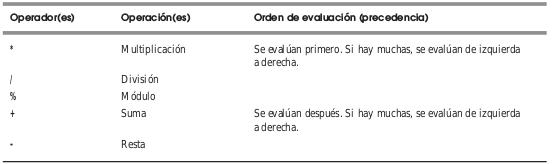
\includegraphics{precedencia-operadores.jpg}
\caption{Precedencia de Operadores}
\end{figure}

\end{frame}

\begin{frame}{Operadores de Igualdad y Relación}

\begin{figure}[htbp]
\centering
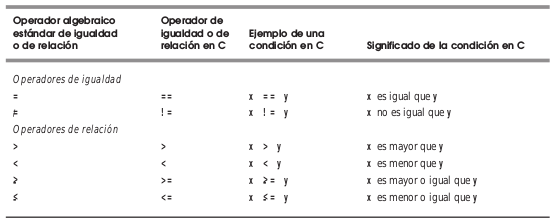
\includegraphics{operadores-igual-rel.jpg}
\caption{Operadores de Igualdad y Relación}
\end{figure}

\end{frame}

\begin{frame}{Ejercicios.}

\begin{itemize}
\itemsep1pt\parskip0pt\parsep0pt
\item
  Hacer un programa que pida dos números y te diga si son iguales o no.
\end{itemize}

\end{frame}

\section{Sentencias de Control}\label{sentencias-de-control}

\begin{frame}[fragile]{Sentencia if}

Permite ejecutar o no una sentencia o bloque, en función de si una
expresión es cierta o no.

\begin{itemize}
\itemsep1pt\parskip0pt\parsep0pt
\item
  Una sentencia:
\end{itemize}

\begin{Shaded}
\begin{Highlighting}[]
\KeywordTok{if} \NormalTok{(expresion)}
    \NormalTok{sentencia;}
\end{Highlighting}
\end{Shaded}

\begin{itemize}
\itemsep1pt\parskip0pt\parsep0pt
\item
  Un bloque:
\end{itemize}

\begin{Shaded}
\begin{Highlighting}[]
\KeywordTok{if} \NormalTok{(expresion)}
    \NormalTok{\{}
    \CommentTok{//bloque}
    \NormalTok{...}
    \NormalTok{\}}
\end{Highlighting}
\end{Shaded}

``expresion'' se construye con operadores lógicos y relacionales.

\end{frame}

\begin{frame}{Diagrama de Flujo if}

\begin{figure}[htbp]
\centering
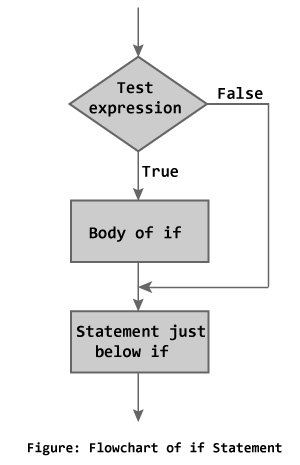
\includegraphics{if.jpg}
\caption{Diagrama de Flujo if}
\end{figure}

\end{frame}

\begin{frame}[fragile]{Sentencia if-else}

Permite ejecutar una sentencia o bloque u otra sentencia o bloque en
función de si una expresión es cierta o no.

\begin{itemize}
\item
\begin{Shaded}
\begin{Highlighting}[]
\KeywordTok{if} \NormalTok{(expresion)}
    \NormalTok{sentencia;}
\KeywordTok{else}
    \NormalTok{sentencia;}
\end{Highlighting}
\end{Shaded}
\item
\begin{Shaded}
\begin{Highlighting}[]
\KeywordTok{if} \NormalTok{(expresion)}
    \NormalTok{\{}
    \CommentTok{//bloque}
    \NormalTok{...}
    \NormalTok{\}}
\KeywordTok{else}
    \NormalTok{sentencia;}
\end{Highlighting}
\end{Shaded}
\item
  Blablabla\ldots{}
\end{itemize}

\end{frame}

\begin{frame}{Diagrama de Flujo if-else}

\begin{figure}[htbp]
\centering
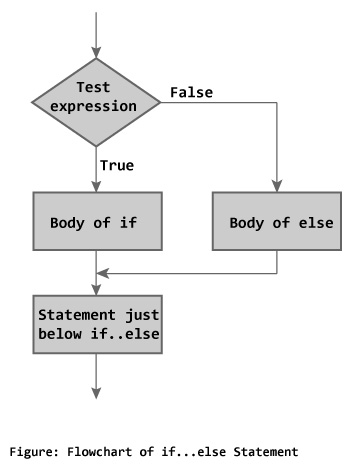
\includegraphics{if-else.jpg}
\caption{Diagrama de Flujo if-else}
\end{figure}

\end{frame}

\begin{frame}[fragile]{Sentencia if e if-else anidados}

Entre las sentencias después de \texttt{if} o \texttt{else} pueden haber
más \texttt{if} e \texttt{if-else}. Por el lado del \texttt{else}:

\begin{Shaded}
\begin{Highlighting}[]
\KeywordTok{if} \NormalTok{(condicion_1)}
    \NormalTok{\{}
    \NormalTok{...}
    \NormalTok{\}}
\KeywordTok{else}
     \KeywordTok{if} \NormalTok{(condicion_2)}
        \NormalTok{\{}
        \NormalTok{...}
        \NormalTok{\}}
    \KeywordTok{else}
         \KeywordTok{if} \NormalTok{(condicion_3)}
            \NormalTok{\{....}
\end{Highlighting}
\end{Shaded}

\end{frame}

\begin{frame}[fragile]{Sentencia if e if-else anidados}

Entre las sentencias después de \texttt{if} o \texttt{else} pueden haber
más \texttt{if} e \texttt{if-else}. Por el lado del \texttt{if}:

\begin{Shaded}
\begin{Highlighting}[]
\KeywordTok{if} \NormalTok{(condicion_1)}
    \NormalTok{\{}
    \KeywordTok{if} \NormalTok{(condicion_2)}
        \NormalTok{\{}
        \NormalTok{...}
        \NormalTok{\}}
    \KeywordTok{else}
        \NormalTok{\{}
        \NormalTok{...}
        \NormalTok{\}}
    \NormalTok{\}}
\KeywordTok{else} \NormalTok{...}
\end{Highlighting}
\end{Shaded}

\end{frame}

\begin{frame}[fragile]{Diagrama de Flujo if-else-anidados}

Pero tambien puede haber más \texttt{if} e \texttt{if-else} por ambos
lados\ldots{}

\begin{Shaded}
\begin{Highlighting}[]
\KeywordTok{if} \NormalTok{(condicion_1)}
    \NormalTok{\{}
    \KeywordTok{if} \NormalTok{(condicion_2)}
        \NormalTok{\{}
        \NormalTok{...}
        \NormalTok{\}}
    \KeywordTok{else}
        \NormalTok{\{}
        \NormalTok{...}
        \NormalTok{\}}
    \NormalTok{\}}
\KeywordTok{else}    
    \NormalTok{\{...\}}
\end{Highlighting}
\end{Shaded}

\end{frame}

\begin{frame}{Diagrama de Flujo if-else-anidados}

\begin{figure}[htbp]
\centering
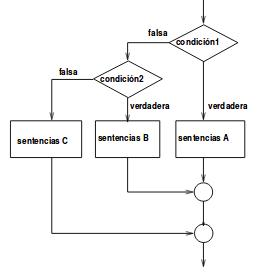
\includegraphics{if-else-anidados.jpg}
\caption{Diagrama de Flujo if-else-anidados por el lado del else}
\end{figure}

\end{frame}

\begin{frame}{Diagrama de Flujo if-else-anidados}

\begin{figure}[htbp]
\centering
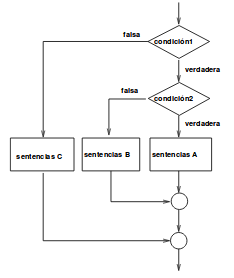
\includegraphics{if-else-anidados-2.jpg}
\caption{Diagrama de Flujo if-else-anidados por el lado del if}
\end{figure}

\end{frame}

\begin{frame}{Ejercicios}

\begin{itemize}
\item
  Hacer un programa que diga si un caracter es vocal o consonante.
\item
  Hacer un programa que diga el número más grande entre cuatro números.
\end{itemize}

\end{frame}

\begin{frame}[fragile]{Sentencia Switch}

Es como tener varios \texttt{if-else} restringiendo la condición a la
comparación de la igualdad entre la expresión y constantes.

\begin{itemize}
\item
  Switch

\begin{Shaded}
\begin{Highlighting}[]
\KeywordTok{switch} \NormalTok{(expresion)}
    \NormalTok{\{}
    \KeywordTok{case} \NormalTok{cte1: ...}
        \KeywordTok{break}\NormalTok{;}
    \KeywordTok{case} \NormalTok{cte2: ...}
        \KeywordTok{break}\NormalTok{;}
    \NormalTok{...}
    \KeywordTok{default}\NormalTok{: ...}
    \NormalTok{\}}
\end{Highlighting}
\end{Shaded}
\end{itemize}

\end{frame}

\begin{frame}[fragile]{Sentencia Switch}

\begin{itemize}
\item
  if

\begin{Shaded}
\begin{Highlighting}[]
\KeywordTok{if} \NormalTok{(expresion == cte1)}
    \NormalTok{\{}
    \NormalTok{...}
    \NormalTok{\}}
\KeywordTok{else}
    \KeywordTok{if} \NormalTok{(expresion == cte2)}
        \NormalTok{\{}
        \NormalTok{...}
        \NormalTok{\}}
\NormalTok{...}
        \KeywordTok{else}
            \NormalTok{...}
\end{Highlighting}
\end{Shaded}
\end{itemize}

\end{frame}

\begin{frame}{Sentencia Switch}

Cosas a considerar

\begin{itemize}
\item
  Si se omite break se ejecuta todo el código que siga hasta encontrar
  el siguiente.
\item
  La expresión es de tipo entero o caracter.
\item
  Después de \texttt{case} solo pueden ir constantes de este tipo.
\item
  La condición es, implícitamente, la comparación a igualdad entre
  \texttt{expresion} y las constantes. No se pueden hacer otro tipo de
  comparación.
\end{itemize}

\end{frame}

\begin{frame}{Ejercicios}

\begin{itemize}
\itemsep1pt\parskip0pt\parsep0pt
\item
  Hacer una calculadora, la calculadora debe de recibir dos numeros tipo
  float y un caracter para decidir que operación se quiere hacer. Se le
  debe de mostrar al usuario un menú de opciones para realizar la
  operación. Acto seguido el usuario ingresa los números y el programa
  devuelve el resultado.
\end{itemize}

\end{frame}
